Nulla sit amet lectus et sapien pretium eleifend. Nam pharetra, urna et porttitor auctor, ipsum sapien rutrum ligula, id porttitor sem lacus nec nulla. Donec imperdiet iaculis urna ut dapibus. Maecenas pulvinar semper ipsum sagittis fermentum. Fusce bibendum vestibulum volutpat. Vestibulum ante ipsum primis in faucibus orci luctus et ultrices posuere cubilia curae.

\begin{defi}
(Exemplo) Sed sagittis nisl enim, eu pretium metus pharetra quis. Nunc eleifend lectus a nisl ultricies finibus. Morbi ut ultricies neque. Curabitur sagittis vestibulum mi, nec auctor diam ultricies id. Morbi tincidunt nisl leo, sed efficitur est mattis vitae. Aliquam erat volutpat. Nam fringilla tristique orci rutrum tempus. 
\end{defi}

Maecenas eu volutpat turpis, in blandit nunc. Aliquam porttitor tortor eu diam mollis, et facilisis eros porttitor. Aenean purus ligula, molestie nec neque vestibulum, sagittis faucibus lectus. Cras sit amet ante sed diam ornare ultrices vitae ac justo. Nunc nec imperdiet est, eget bibendu

\begin{figure}[!htb]
    \centering
    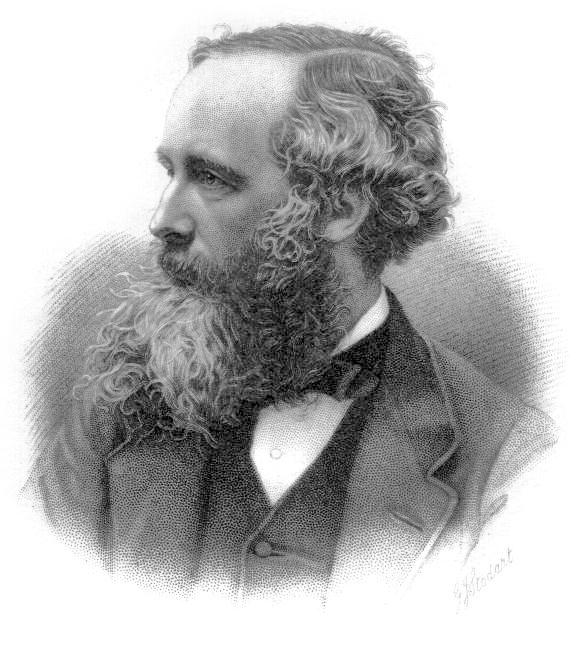
\includegraphics[width=0.3\linewidth]{James_Clerk_Maxwell_big.jpg}
    \caption{James Maxwell}
    \label{fig:maxwell}
\end{figure}

\newpage

Nulla sit amet lectus et sapien pretium eleifend. Nam pharetra, urna et porttitor auctor, ipsum sapien rutrum ligula, id porttitor sem lacus nec nulla. 

\begin{description}
    \item[Lei de Gauss]
    $$\nabla \cdot \textbf{E} = \frac{\rho}{\epsilon_{0}}$$
    
    \item[Lei de Gauss para o Magnetismo]
    $$\nabla \cdot \textbf{B} = 0$$
    
    \item[Lei de Faraday para Indução]
    $$\nabla \times \textbf{E} = -\frac{\partial \textbf{B}}{\partial t}$$
    
    \item[Lei circular de Ampère]
    $$\nabla \times \textbf{B} = \mu_{0}\left(\textbf{J} + \epsilon_{0}\frac{\partial \textbf{E}}{\partial t} \right)$$
\end{description}

\newpage